% 第五章：实验评估（精修投稿版——完整保留真实与合成主证据、消融与 Uniform-Narrow 适用边界，消除重复表格）
\section{Experimental Evaluation}
\label{sec:eval}

\subsection{Experimental Setup}
\label{subsec:eval_setup}

\paragraph{Hardware and Protocol.}
Experiments run in isolated Linux containers with {AMD EPYC 9654} ({Zen~4}) CPUs, each restricted via cgroups to 32 logical CPUs and $60$\,GiB RAM (swap off, {THP} \texttt{never} with $4$\,KiB pages, one job per container, native {AVX-512F}/{AVX2+FMA} Rust builds, $M = 16, M_0 = 32, L_c = 128, \alpha = 1.2$, $32$ build threads). In the main comparisons, the cold FP32 rerank store ($3{,}072$\,MB at $N=1\text{M}, D=768$) resides in RAM alongside the hot navigation index.
Following standard ANN evaluation practice~\cite{aumuller2020annbenchmarks,simhadri2022results}, we report throughput tables and curves from the first build per configuration (seed \texttt{12345} where supported, upstream randomization for HDB). Each thread count uses the fastest measured point meeting its recall target. A repeatability check over $210$ operating points and three seeds found at most $0.22$\,pp variation in recall and $\pm2.64\%$ in Core QPS at $99\%$ recall on Cohere ($\pm0.20\%$ on MERU).

\paragraph{Fixed Parameters and Operating-Point Selection.}
Full-method sweeps scan $L\in\{32,\allowbreak64,\allowbreak96,\allowbreak128,\allowbreak192,\allowbreak200,\allowbreak208,\allowbreak256,\allowbreak384,\allowbreak512,\allowbreak768,\allowbreak1024,\allowbreak1536,\allowbreak2048\}$, $B \in \{32, 64, 128\}$ ($B \le L$), and $\Delta_0 \in \{0.08, 0.12, 0.20\}$ (controls add full-pool reranking and sketch-off paths), with fixed build/purity/\textsc{CJ-Gate} constants across datasets (settings in supplemental material).
{MERU-1M}, {OpenAI-1536}, {WordNet-Hazy}, and the synthetic datasets use disjoint $2{,}000$-query tuning sets. For {Cohere-1M}, we use the $1{,}000$ public {VectorDBBench} queries and compute exact top-10 neighbors over the mapped database in FP64. For each method and thread count, the {Cohere-1M} frontier reports the highest measured QPS meeting each recall threshold on these queries.

\begin{table}[t]
  \centering
  \caption{Hyperbolic benchmarks in $\Bunit$ ($c=1$), ordered from native to mapped real workloads and clustered to isotropic synthetic stress sets.}
  \label{tab:datasets}
  \footnotesize
  \setlength{\tabcolsep}{3pt}
  \begin{tabularx}{\linewidth}{@{}lrrr>{\raggedright\arraybackslash}X@{}}
    \toprule
    \textbf{Dataset} & $N$ & $D$ & $|Q|$ & \textbf{Manifold Geometry} \\
    \midrule
    MERU-1M~\cite{astrmira2026meruimagenet1m} & 1,000K & 512 & 10,000 & Native {Lorentz}$\to\Bunit$ multimodal \\
    WordNet-Hazy & 83.9K & 20 & 2,000 & Native {Lorentz}$\to\mathbb{B}_1^{20}$ taxonomy \\
    Cohere-1M & 1,000K & 768 & 1,000 & Mapped Wikipedia ($\exp_0^1$, $\rho_{0.01}=1.44$) \\
    OpenAI-1536 & 990K & 1,536 & 8,000 & Mapped DBpedia ($\exp_0^1$, $\text{med}\,\rho=2.0$) \\
    \midrule
    Clustered-Narrow & 1,000K & 512 & 2,000 & $256$ tight cones, $\rho \in [3.9, 4.1]$ \\
    Clustered-Wide & 1,000K & 512 & 2,000 & $256$ tight cones, $\rho \in [0.4, 6.0]$ \\
    Uniform-Narrow & 1,000K & 512 & 2,000 & Isotropic $\mathbb{S}^{511}$, $\rho \in [3.9, 4.1]$ \\
    Uniform-Wide & 1,000K & 512 & 2,000 & Isotropic $\mathbb{S}^{511}$, $\rho \in [0.4, 6.0]$ \\
    \bottomrule
  \end{tabularx}
\end{table}

\paragraph{Benchmarks and Baselines.}
Table~\ref{tab:datasets} lists the eight primary $\Bunit$ ($c=1$) workloads, leading with native hyperbolic embeddings.
To evaluate native hyperbolic search at million-vector scale, we constructed and released \textbf{MERU-1M}~\cite{astrmira2026meruimagenet1m} by encoding {ImageNet} images with the frozen {MERU ViT-small} encoder~\cite{desai2023meru}.
The benchmark provides one million 512-dimensional database vectors in Poincar\'e coordinates~\eqref{eq:lorentz_isometry}, disjoint sets of $2{,}000$ tuning and $10{,}000$ test queries, and exhaustive FP64 geodesic ground truth.
\textbf{WordNet-Hazy} maps $83{,}943$ $20$D {Lorentz} {WordNet} embeddings into $\mathbb{B}_1^{20}$ ($\le 2.53\times 10^{-15}$ max numerical error).
\textbf{Cohere-1M} and \textbf{OpenAI-1536} serve as derivative radial-$\tanh$ stress tests mapped from database mean $\bar{x}$ via $\Phi(x) = \tanh\bigl(\frac{s}{2}\|x - \bar{x}\|_2\bigr)\frac{x - \bar{x}}{\|x - \bar{x}\|_2}$ ($s = 2/\operatorname{median}_i(\|x_i - \bar{x}\|_2)$, clamped at $1 - 10^{-6}$ for $\rho_{0.50} = 2.0$).
On \textbf{Cohere-1M} ($s = 0.2644$, zero clipped points), norm concentration creates a hollow shell with base depths $[0.98, 3.39]$ ($\rho_{0.01}=1.45, \rho_{0.99}=2.69$) and query depths $[1.25, 2.98]$ ($\rho_{0.01}=1.44$).
\textbf{OpenAI-1536} unit-normalizes \texttt{text-embedding-3-large} {DBpedia} vectors before centering and $\Phi(x)$ ($s = 2.093$, $8{,}000$ test + $2{,}000$ tuning queries).
Each synthetic set has one million 512D vectors. Crossing angular concentration (256 tight cones or isotropic directions) with radial support ($[3.9,4.1]$ or $[0.4,6.0]$) lets us vary either factor independently.

Internally, \textbf{Polar-FP32/SQ8} use unquantized FP32 or 8-bit directions in build and search, \textbf{SameGraph-FP32/SQ8} freeze the 2-bit graph and swap only search directions, and 2-bit progression spans \textbf{\rquiver{}-Split} (no chord swaps, \texttt{HotSmPage}, or \texttt{SymSketch256}) $\to$ \textbf{\rquiver{}-Core} (adding all three under global {SM}) $\to$ \textbf{\rquiver{}} (enabling \texttt{ResidualConeDict} and \textsc{CJ-Gate}, whereas \textbf{Global-SM} disables cone rescue, \textsc{CJ-Gate}, and stabilized sketch margins).
We report \textbf{Exact-RobustPrune}~\cite{subramanya2019diskann,prokhorenkova2022hyperbolic} on {Cohere-1M} to test exact geodesic pruning on a hollow shell ($M/L_c=16/128$, $L\le2{,}048$). We test \textbf{HyperspaceDB}~\cite{glukhota2026hyperspacedb} (HDB, commit \texttt{89d0406}, Nov.\ 9, 2026, native AVX-512F Poincar\'e HNSW, FP32/FP64 dynamic/flat), \textbf{Faiss}~\cite{douze2024faiss} (\texttt{faiss-cpu 1.16.0}, \texttt{IndexHNSWFlat}), and \textbf{Milvus}~\cite{wang2021milvus} (Standalone 3.0.5, centered-IP HNSW) at $M/L_c=16/128$ and $32/256$ with 18 $ef$ values up to $4{,}096$. In this sweep HDB and Milvus return native top-10. Faiss uses FP64 rerank budgets $B\in\{0,32,128\}$ for centered IP and raw Lorentz-IP, and $B\in\{32,128\}$ for direction search. For Lorentz coordinates $(t,\mathbf{s})$, centered IP stores $(t_v-\bar t,\mathbf{s}_v)$ and queries with $(-t_q,\mathbf{s}_q)$, where $\bar t$ is the database mean time coordinate. Their dot product preserves Lorentz ordering up to the query-only offset $t_q\bar t$ before rounding. HNSW builds links using ordinary inner products between stored vectors.

\subsection{Index Construction and Polar Representations}
\label{subsec:eval_repr}

\begin{table*}[t]
  \centering
  \caption{Real-data throughput and Cohere-1M representation controls. Each configuration uses one build and 32 construction threads.}
  \label{tab:zen4_repr}
  \footnotesize
  \setlength{\tabcolsep}{3.5pt}
  \begin{tabular*}{\linewidth}{@{\extracolsep{\fill}}llrrrrrrrrrrrr@{}}
    \toprule
    & & \textbf{Build} & \textbf{Hot Nav} & \textbf{Zero-In} & \multicolumn{3}{c}{\textbf{Recall@10 $\ge 98\%$}} & \multicolumn{3}{c}{\textbf{Recall@10 $\ge 99\%$}} & \multicolumn{3}{c}{\textbf{Recall@10 $\ge 99.5\%$}} \\
    \cmidrule(lr){6-8}\cmidrule(lr){9-11}\cmidrule(lr){12-14}
    \textbf{Dataset} & \textbf{Method} & \textbf{32T\,(s)} & \textbf{(MB)} & \textbf{Islands} & \textbf{1T QPS} & \textbf{p99} & \textbf{24T QPS} & \textbf{1T QPS} & \textbf{p99} & \textbf{24T QPS} & \textbf{1T QPS} & \textbf{p99} & \textbf{24T QPS} \\
    \midrule
    \multicolumn{14}{@{}l}{\textbf{(a) Real-world workloads: native hyperbolic (MERU-1M, WordNet-Hazy) and mapped hyperbolic (Cohere-1M, OpenAI-1536)}} \\
    MERU-1M & \textbf{\rquiver{}} & 25.7 & 516.8$^*$ & 0 & 2,547 & 0.50 & 53,483 & 2,547 & 0.50 & 53,483 & 1,669 & 0.81 & 36,092 \\
    WordNet-Hazy & \textbf{\rquiver{}} & 1.5 & 32.8$^*$ & 0 & 4,130 & 0.29 & 89,847 & 3,089 & 0.38 & 65,405 & 2,341 & 0.49 & 52,371 \\
    Cohere-1M & \textbf{\rquiver{}} & 35.0 & 517.0$^*$ & 0 & 2,907 & 0.41 & 58,162 & 1,930 & 0.62 & 42,466 & 738 & 1.65 & 17,137 \\
    OpenAI-1536 & \textbf{\rquiver{}} & 43.6 & 765.6$^*$ & 0 & 1,378 & 1.03 & 25,725 & 792 & 1.81 & 14,731 & 481 & 3.05 & 9,094 \\
    \midrule
    \multicolumn{14}{@{}l}{\textbf{(b) Controlled internal representation comparison on Cohere-1M (end-to-end 1T + 24T)}} \\
    \multirow{5}{*}{Cohere-1M}
     & Polar-FP32 & 197.7 & 3,373.0$^\ddagger$ & 0 & 1,048 & 1.17 & 15,063 & 457 & 2.63 & 7,004 & 265 & 4.33 & 3,928 \\
     & Polar-SQ8 & 68.3 & 1,069.0$^\ddagger$ & 0 & 1,818 & 0.75 & 36,304 & 858 & 1.56 & 16,488 & 396 & 3.25 & 7,353 \\
     & \rquiver{}-Split & \textbf{32.2} & \textbf{485.0} & 628 & 2,765 & 0.43 & 56,828 & 1,739 & 0.72 & 37,747 & 617 & 1.84 & 14,393 \\
     & \rquiver{}-Core & 32.8 & 517.0$^*$ & 0 & \textbf{3,800} & \textbf{0.31} & \textbf{73,861} & \textbf{2,003} & \textbf{0.59} & \textbf{46,796} & 687 & \textbf{1.64} & 16,029 \\
     & \textbf{\rquiver{}} & 35.0 & 517.0$^*$ & \textbf{0} & 2,907 & 0.41 & 58,162 & 1,930 & 0.62 & 42,466 & \textbf{738} & 1.65 & \textbf{17,137} \\
    \bottomrule
  \end{tabular*}
  \par\vspace{1pt}
  {\scriptsize \textit{Note:} Hot Nav measures active traversal memory (excluding the shared $3{,}072.0$\,MB cold FP32 rerank store for 2-bit/SQ8); 1T p99 in ms. $^*$Includes \texttt{HotSmPage} and sketch. The corresponding split layouts without sketches use $420.8$, $26.1$, $485.0$, and $670.6$\,MB on MERU, WordNet-Hazy, Cohere, and OpenAI, respectively. $^\ddagger$Active SQ8/FP32 totals ($+8.0$\,MB inv.\ norms; raw benchmark counters kept unaccessed $192.0$\,MB 2-bit bitplanes, reading $1{,}261.0$/$3{,}565.0$\,MB; Table~\ref{tab:node_layout}). The $98\%$ and $99\%$ MERU entries select the same configuration.}
\end{table*}

On {MERU-1M}, $(L,B,\Delta_0)=(128,128,0.20)$ gives $99.252\%$ recall at $2{,}547$/$53{,}483$\,QPS (1T/24T). At $L=256$, recall is $99.758\%$ at $1{,}669$/$36{,}092$\,QPS. All four real-data graphs have zero islands and zero active cones (Table~\ref{tab:zen4_repr}a).

On {Cohere-1M}, construction takes $35.0$\,s for \rquiver{} and $197.7$\,s for Polar-FP32. Hot navigation occupies $517$ versus $3{,}373$\,MB ($3{,}589$\,MB including cold vectors for \rquiver{}). At $98\%$, Core selects $(64,64,0.20)$ and full \rquiver{} selects $(96,64,0.12)$. At the latter setting Core serves $3{,}230$\,QPS at $98.24\%$ and the full method $2{,}907$ at $98.27\%$. Core also leads at the $99\%$ target. The full method leads at $99.5\%$ on both thread counts.

\subsection{Comparison with Hyperbolic and Flat-Proxy Engines}
\label{subsec:eval_external}

\begin{table*}[t]
  \centering
  \caption{Measured comparison of \rquiver{} and external baselines on native {MERU-1M} and mapped {Cohere-1M} (Zen~4, 32 build threads; 1T and 24T).}
  \label{tab:external_baselines}
  \scriptsize
  \setlength{\tabcolsep}{1.5pt}
  % 原生双曲（MERU-1M 优先）与高维空心映射（Cohere-1M）外部对照分区精排总表（消除无关全空占位列）
\begin{tabular*}{\linewidth}{@{\extracolsep{\fill}}llrrrrrrrrrrrrr@{}}
\multicolumn{15}{@{}l}{\textbf{(a) MERU-1M (Native Hyperbolic, $512$D, $10{,}000$ queries; main-sweep methods reaching $99.5\%$ Recall@10)}} \\
\toprule
 & & \textbf{Build} & \textbf{Peak} & \multicolumn{5}{c}{\textbf{1-Thread QPS at Recall@10}} & \textbf{1T p99} & \multicolumn{5}{c}{\textbf{24-Thread QPS at Recall@10}} \\
\cmidrule(lr){5-9}\cmidrule(lr){11-15}
\textbf{Method} & \textbf{$M/L_c$} & \textbf{32T\,(s)} & \textbf{Rec@10} & \textbf{$\ge90\%$} & \textbf{$\ge95\%$} & \textbf{$\ge98\%$} & \textbf{$\ge99\%$} & \textbf{$\ge99.5\%$} & \textbf{(ms)} & \textbf{$\ge90\%$} & \textbf{$\ge95\%$} & \textbf{$\ge98\%$} & \textbf{$\ge99\%$} & \textbf{$\ge99.5\%$} \\
\midrule
\textbf{\rquiver{}} & 16/128 & \textbf{25.7} & 99.983\% & \textbf{5,846} & \textbf{4,521} & \textbf{2,547} & \textbf{2,547} & \textbf{1,669} & \textbf{0.50} & \textbf{94,846} & \textbf{94,846} & \textbf{53,483} & \textbf{53,483} & \textbf{36,092} \\
HDB FP32 flat & 16/128 & 87.6 & 99.947\% & 3,187 & 2,184 & 1,579 & 1,296 & 966 & 1.15 & 26,235 & 26,235 & 19,434 & 15,890 & 11,699 \\
HDB FP32 dynamic & 16/128 & 86.5 & 99.947\% & 3,136 & 2,103 & 1,493 & 1,188 & 875 & 1.27 & 30,015 & 30,015 & 18,413 & 13,780 & 11,038 \\
HDB FP64 dynamic & 32/256 & 631.4 & 99.955\% & 615 & 428 & 281 & 196 & 165 & 8.83 & 9,588 & 9,588 & 6,121 & 4,098 & 3,414 \\
HDB FP64 flat & 32/256 & 633.9 & 99.707\% & 480 & 320 & 186 & 93 & 46 & 21.68 & 6,362 & 6,362 & 4,039 & 1,933 & 925 \\
Faiss direction & 16/128 & 48.8 & \textbf{100.000\%} & 3,460 & 1,814 & 1,480 & 1,078 & 1,078 & 1.30 & 43,798 & 43,798 & 19,883 & 14,967 & 9,866 \\
Faiss centered IP & 32/256 & 99.2 & 99.988\% & 4,312 & 2,800 & 1,903 & 1,059 & 872 & 1.43 & 33,189 & 33,189 & 22,488 & 13,005 & 9,349 \\
Milvus centered IP & 32/256 & 271.6 & 99.991\% & 297 & 297 & 297 & 260 & 233 & 5.30 & 1,208 & 1,208 & 1,208 & 1,130 & 1,088 \\
\bottomrule
\end{tabular*}
\par\smallskip
\begin{tabular*}{\linewidth}{@{\extracolsep{\fill}}lrrrrrr@{}}
\multicolumn{7}{@{}l}{\textbf{MERU-1M log-map and quantized controls ($99\%$ validation target, 10,000 test queries)}}\\
\toprule
& \multicolumn{3}{c}{1 thread} & \multicolumn{3}{c}{24 threads}\\
\cmidrule(lr){2-4}\cmidrule(l){5-7}
Method & Recall@10 (\%) & QPS & p99 (ms) & Recall@10 (\%) & QPS & p99 (ms)\\
\midrule
Faiss FP32 (log-map $L_2$) & 99.059 & 2,136 & 0.65 & 99.150 & 15,103 & 2.61\\
Faiss SQ8 (log-map $L_2$) & 99.119 & 1,220 & 1.07 & 99.119 & 26,786 & 1.28\\
Milvus SQ8 (centered IP) & 99.405 & 73 & 20.75 & 99.716 & 587 & 115.23\\
HDB SQ8 (Poincar\'e, FP64 rerank) & 99.224 & 763 & 1.85 & 99.224 & 13,620 & 2.52\\
Tangent 2-bit (paired engine) & 99.107 & 1,510 & 0.99 & 99.107 & 35,813 & 0.99\\
\rquiver{} 2-bit (paired engine) & 99.248 & 2,311 & 0.55 & 99.247 & 50,848 & 0.60\\
\bottomrule
\end{tabular*}

\par\vspace{3pt}
\begin{tabular*}{\linewidth}{@{\extracolsep{\fill}}llrrrrrrrrrr@{}}
\multicolumn{12}{@{}l}{\textbf{(b) Cohere-1M (Mapped Hollow Shell, $768$D, $1{,}000$ queries; baselines reaching $\ge95\%$ Recall@10)}} \\
\toprule
 & & \textbf{Build} & \textbf{Peak} & \multicolumn{4}{c}{\textbf{1-Thread QPS at Recall@10}} & \multicolumn{4}{c}{\textbf{24-Thread QPS at Recall@10}} \\
\cmidrule(lr){5-8}\cmidrule(lr){9-12}
\textbf{Method} & \textbf{$M/L_c$} & \textbf{32T\,(s)} & \textbf{Rec@10} & \textbf{$\ge90\%$} & \textbf{$\ge95\%$} & \textbf{$\ge98\%$} & \textbf{$\ge99\%$} & \textbf{$\ge90\%$} & \textbf{$\ge95\%$} & \textbf{$\ge98\%$} & \textbf{$\ge99\%$} \\
\midrule
\textbf{\rquiver{}} & 16/128 & \textbf{35.0} & \textbf{99.700\%} & \textbf{4,939} & \textbf{4,939} & \textbf{2,907} & \textbf{1,930} & \textbf{96,584} & \textbf{96,584} & \textbf{58,162} & \textbf{42,466} \\
Faiss centered IP & 32/256 & 167.3 & 98.910\% & 1,652 & 830 & 127 & \missing & 10,717 & 10,717 & 1,660 & \missing \\
Milvus centered IP & 32/256 & 361.7 & 98.690\% & 252 & 238 & 76 & \missing & 1,115 & 1,115 & 999 & \missing \\
HDB FP32 dynamic & 32/256 & 414.8 & 96.780\% & 839 & 290 & \missing & \missing & 3,416 & 3,416 & \missing & \missing \\
HDB FP32 flat & 32/256 & 416.3 & 96.670\% & 946 & 279 & \missing & \missing & 3,656 & 3,656 & \missing & \missing \\
\bottomrule
\end{tabular*}

  \par\vspace{1pt}
  {\scriptsize HDB = HyperspaceDB. Dashes mark unmet targets ($ef\le4{,}096$). Build and $M/L_c$ refer to the $99\%$ point or the highest recall reached. The 1T p99 is from the selected $99\%$ point. The paired-engine rows use a separate, sequentially timed comparison with validation-selected budgets. For \rquiver{}, $(L,B)$ is $(128,128)$ at 1T and $(128,32)$ at 24T. On Cohere, Exact-RobustPrune peaks at $93.94\%$, HDB FP64 at $94.43\%$, and Faiss direction/raw-IP at $65.17/0.12\%$.}
\end{table*}

\begin{figure*}[t]
  \centering
  \begin{subfigure}[t]{0.328\textwidth}
    \centering
    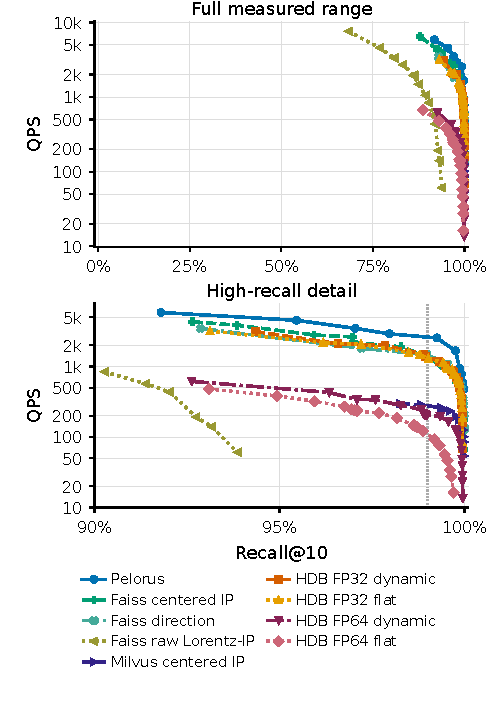
\includegraphics[width=\linewidth]{pareto_meru_1m_1t.pdf}
    \caption{MERU-1M ($512$D, 1 thread)}
    \label{fig:pareto_meru}
  \end{subfigure}\hfill
  \begin{subfigure}[t]{0.328\textwidth}
    \centering
    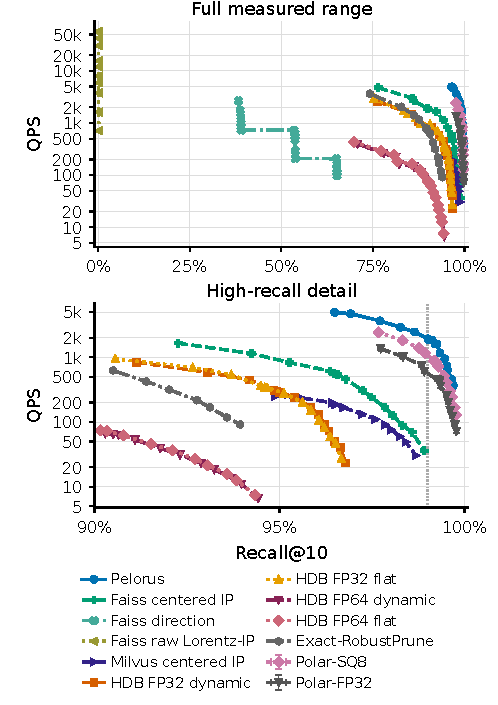
\includegraphics[width=\linewidth]{pareto_cohere_1m_1t.pdf}
    \caption{Cohere-1M ($768$D, 1 thread)}
    \label{fig:pareto_cohere}
  \end{subfigure}\hfill
  \begin{subfigure}[t]{0.30\textwidth}
    \centering
    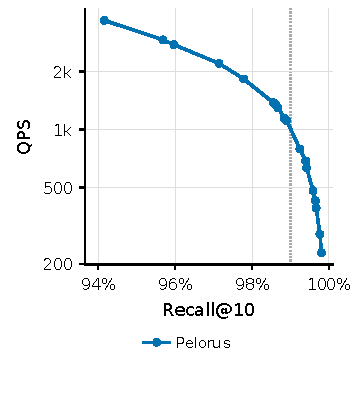
\includegraphics[width=\linewidth]{pareto_openai_1536_1t.pdf}
    \caption{OpenAI-1536 ($1536$D, 1 thread)}
    \label{fig:pareto_openai}
  \end{subfigure}
  \caption{Single-build, single-thread Recall@10--QPS frontiers on Zen~4. Panels (a,b) include external baselines. Panel (c) shows \rquiver{} on mapped {OpenAI-1536}.}
  \label{fig:real_pareto}
\end{figure*}

On native {MERU-1M} at the $99\%$ target, \rquiver{} serves $1.97\times/3.37\times$ the QPS of HDB FP32 flat and $1.19\times/3.54\times$ that of Faiss FP32 log-map $L_2$ HNSW (1T/24T, Table~\ref{tab:external_baselines}). The log-map~\cite{deng2026hyem} uses $ef=128$ with direct top-10 at 1T and 128-candidate reranking at 24T.

\paragraph{Two-bit tangent-space control.}
Both graphs use the same Rayon scheduler, 2-bit {SM} directions, degree bound and FP64 reranker. The tangent graph uses log-map norms, a single entry and isotropic RobustPrune. At $L=B=128$, it serves $2{,}326$\,QPS at $97.837\%$ recall versus $2{,}248$ at $99.248\%$ for \rquiver{} (1T). To reach $99\%$, it doubles $L$ to 256. At the validation-selected budgets, \rquiver{} serves $1.53\times/1.42\times$ its QPS (1T/24T, Table~\ref{tab:external_baselines}), using $516.8$ versus $428.0$\,MB of hot state.

\paragraph{SQ8 graph indices.}
Across both build budgets and layouts ($ef\le4{,}096$), HDB SQ8 direct top-10 peaks at $63.93/51.75\%$ (Poincar\'e/Lorentz). FP64 reranking of 128 candidates raises Poincar\'e SQ8 above $99\%$ at $ef=256$ and Lorentz SQ8 to $96.66\%$. Faiss \texttt{IndexHNSWSQ} and Milvus \texttt{HNSW\_SQ} test both retrieval modes at $M/L_c=16/128$. Faiss uses in-process C++. Milvus includes Python and gRPC.

On mapped {Cohere-1M}, \rquiver{} reaches $99.70\%$ recall. Over the $32/256$ sweeps ($ef\le4{,}096$), centered-IP {Faiss} and {Milvus} peak at $98.91\%$ and $98.69\%$, and HDB FP32 dynamic and flat at $96.78\%$ and $96.67\%$. Log-map HNSW reaches $86.42\%$ on its separate 500-query test subset.

\subsection{Multi-Threaded Scaling Efficiency}
\label{subsec:eval_scaling}

\begin{figure*}[t]
  \centering
  \begin{subfigure}[t]{0.435\textwidth}
    \centering
    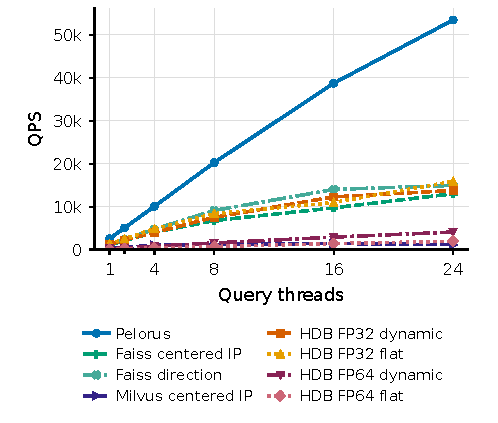
\includegraphics[width=\linewidth]{scaling_meru_1m_r99.pdf}
    \caption{MERU-1M ($\ge 99\%$ Recall)}
    \label{fig:scale_meru}
  \end{subfigure}\hfill
  \begin{subfigure}[t]{0.435\textwidth}
    \centering
    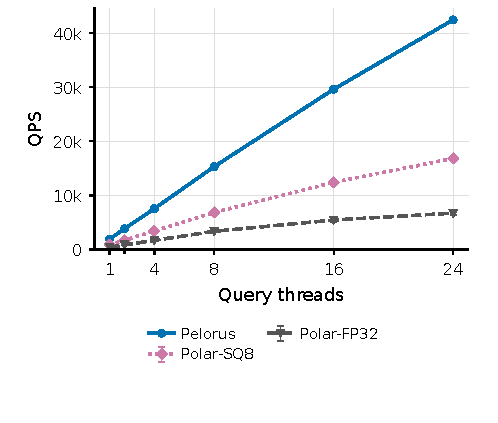
\includegraphics[width=\linewidth]{scaling_cohere_1m_r99.pdf}
    \caption{Cohere-1M ($\ge 99\%$ Recall)}
    \label{fig:scale_cohere}
  \end{subfigure}
  \caption{Single-build scaling from $1$ to $24$ query threads on Zen~4 at Recall@10 $\ge 99\%$.}
  \label{fig:scaling}
\end{figure*}

The single-build scaling curves in Figure~\ref{fig:scaling} give $21.0\times$ speedup from 1T to 24T on {MERU-1M} and $22.0\times$ on {Cohere-1M}. {WordNet-Hazy} and {OpenAI-1536} reach $21.2\times$ and $18.6\times$. On {MERU-1M}, the FP32 {HDB} and {Faiss} baselines scale by $11.6$--$12.3\times$.

\subsection{Page Layout and Cold Storage}
\label{subsec:eval_storage}

On {MERU-1M} ($D=512$), compact packing raises page occupancy from 16 to 21 vertices and cuts allocation from $244.1$ to $186.0$\,MiB. At $(L,B)=(128,64)$ both layouts return identical IDs and scores ($99.249\%$ recall). Throughput moves from $2{,}416$ to $2{,}305$\,QPS at 1T and from $47{,}470$ to $51{,}088$ at 24T. On $65{,}536$-point MERU probes, allocation falls from $16.00$ to $10.24$\,MiB at $D=384$ and from $32.00$ to $21.34$ at $D=1024$. On {Cohere-1M}, both layouts use $244.1$\,MiB. Compact/default 24T throughput is $41{,}336/53{,}323$\,QPS at $(128,64)$ and $30{,}123/32{,}965$ at $(256,128)$. Both share a page translation per record. Packing also changes cache-line placement and address calculation. Hardware miss counters were unavailable. On $20$D {WordNet-Hazy}, compact pages use $6.43$ versus $10.25$\,MiB. Sharing cold FP32 vectors for navigation instead cuts RSS from $70.5$ to $63.9$\,MiB, raises recall from $97.340$ to $99.980\%$ and lowers 1T QPS from $4{,}578$ to $4{,}076$.

\begin{table}[t]
  \centering
  \caption{Cold reranking on {MERU-1M}. The 2-bit navigation graph stays in RAM. All rows use 24 threads, a 512\,MiB SSD cache and $\Delta_0=0.20$. The last column gives SSD bytes read per timed query in KiB.}
  \label{tab:meru_ssd}
  \footnotesize
  \setlength{\tabcolsep}{3pt}
  \begin{tabular}{@{}llrrrr@{}}
    \toprule
    Cold encoding & $L/B$ & Recall@10 & QPS & p99 (ms) & KiB/q \\
    \midrule
    FP32            & 512/128 & 99.917\% & 1,886 & 48.78 & 670.85 \\
    Cartesian FP16  & 512/128 & 99.902\% & 3,282 & 17.26 & 358.32 \\
    Polar FP16      & 512/128 & 99.902\% & 3,270 & 16.83 & 361.73 \\
    \midrule
    Centered SQ8    & 64/64 & 97.519\% & 23,760 & 4.48 & 44.31 \\
    Centered SQ4    & 64/64 & 90.123\% & 33,823 & 4.09 & 21.24 \\
    \bottomrule
  \end{tabular}
\end{table}

For SSD reranking we fix one graph, tune on $2{,}000$ queries, then time each condition once on $10{,}000$ test queries after 200 warmups. Batched \texttt{io\_uring} reads have a 32\,MiB in-flight budget. Polar FP16 and centered SQ4 retain an FP64 radius. At $L=512$, both FP16 formats nearly halve SSD traffic while retaining $99.902\%$ recall (Table~\ref{tab:meru_ssd}). At $L=64$, SQ4 reads $52\%$ fewer bytes per query than SQ8 and serves $42\%$ more queries per second at a cost of $7.396$ recall points. The highest SQ4 recall among the 43 configurations retested is $91.240\%$.

At $99.917\%$ recall and 24T, offloading cold FP32 to SSD with 128\,MiB cache cuts RSS from $2.573$ to $0.825$\,GiB and QPS from $22{,}822$ to $1{,}308$. At $(164,64)$, centered SQ8 gives identical top-10 across RAM and both SSD caches ($99.003\%$ recall). RAM serves $51{,}040$\,QPS (p99 $0.62$\,ms, RSS $1.155$\,GiB). Increasing the cache from 128 to 512\,MiB cuts reads/query from $103.35$ to $10.00$, raises QPS from $2{,}749$ to $20{,}136$ and lowers p99 from $23.87$ to $7.23$\,ms. RSS rises from $0.839$ to $1.228$\,GiB.

\subsection{Geometry and Execution Ablations}
\label{subsec:eval_ablation}

\begin{figure*}[t]
  \centering
  \begin{subfigure}[t]{0.435\linewidth}
    \centering
    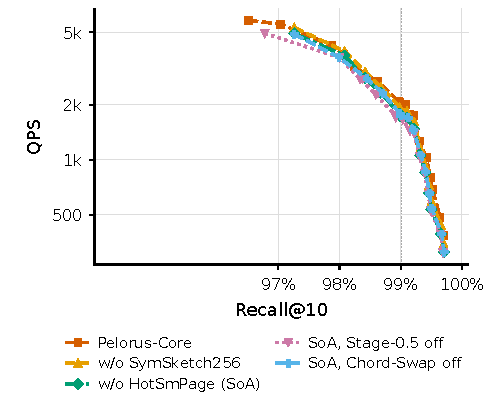
\includegraphics[width=\linewidth]{ablation_geometry_cohere_1m.pdf}
    \caption{Cohere-1M, topology and search}
    \label{fig:abl_geom}
  \end{subfigure}\hfill
  \begin{subfigure}[t]{0.435\linewidth}
    \centering
    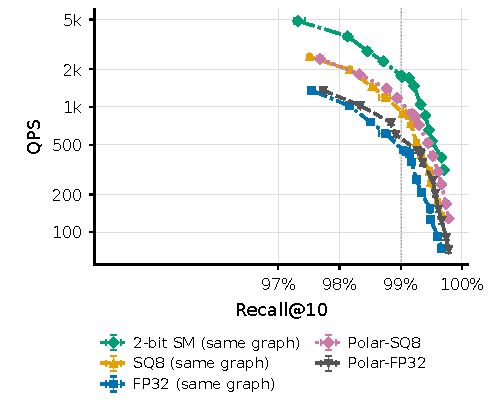
\includegraphics[width=\linewidth]{ablation_representation_cohere_1m.pdf}
    \caption{Cohere-1M, search representation}
    \label{fig:abl_repr}
  \end{subfigure}
  \par\smallskip
  \begin{subfigure}[t]{0.89\linewidth}
    \centering
    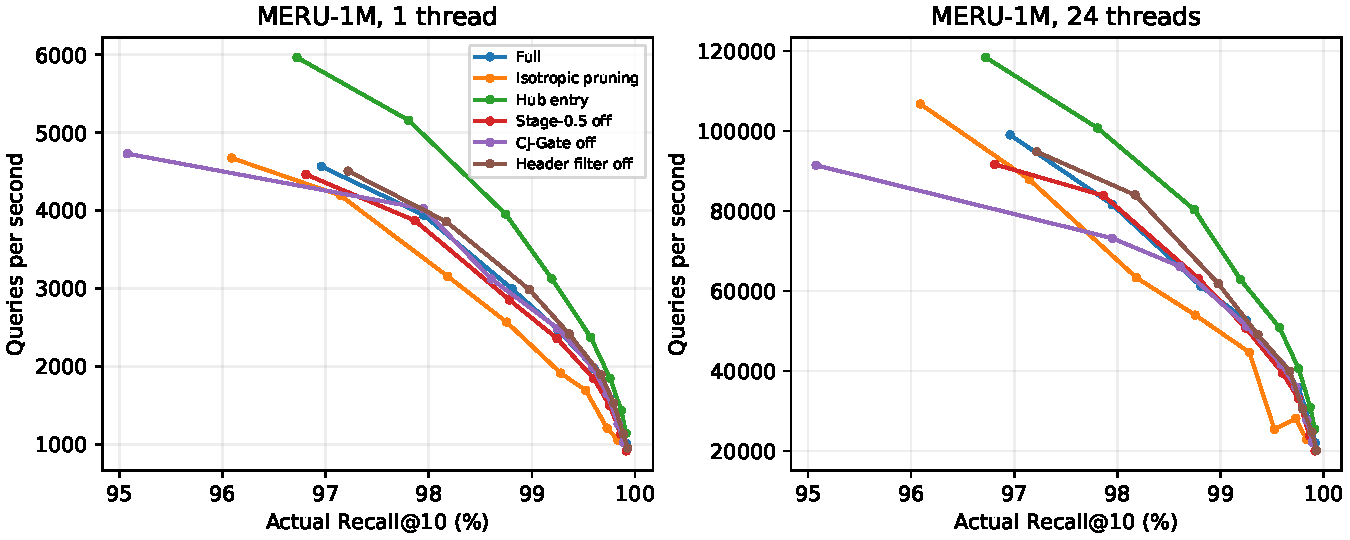
\includegraphics[width=\linewidth]{meru_ablation.pdf}
    \caption{MERU-1M, topology and search at eight fixed budgets.}
    \label{fig:abl_native}
  \end{subfigure}
  \caption{Component ablations on the first build. The upper panels give single-thread frontiers on {Cohere-1M}. The lower panels give measured recall and throughput at eight fixed budgets on {MERU-1M}.}
  \label{fig:ablation_pdf}
\end{figure*}

\paragraph{Cohere-1M}
With the Core engine and 16 budgets, QuadriPrune reaches $99\%$ at $1{,}957$\,QPS versus $426$ for the earlier two-pass policy ($L=192/1{,}536$, $B=64$). At $(192,64)$, removing the ring lowers recall from $99.00\%$ to $97.09\%$ (peak $98.74\%$). Disabling its shield gives $98.99\%$, removing the geodesic channel $99.41\%$, and removing both elevators $99.23\%$.

A simpler graph selects up to 16 of 32 links by angular diversity alone, then uses the same depth-aware refill, repair, entries and scoring. Across three paired rebuilds, QuadriPrune delivers $12$--$15\%$ more QPS at the $99\%$ target. At $99.5\%$ the angular quota delivers $35$--$66\%$ more QPS, reaching the target at $L=384$ versus $768$--$1{,}024$ ($B=128$).

At $99\%$ recall, page co-location raises single-thread throughput from $1{,}701$ to $1{,}850$\,QPS, and the sketch raises it to $2{,}003$ (Figure~\ref{fig:abl_geom}). On the split-array path, disabling \textsc{Stage-0.5} gives $1{,}665$/$391$\,QPS at $99/99.5\%$ versus $1{,}701$/$535$ with it. Chord repair connects 521 zero-in-degree vertices. In the 32-query header traces, the default sketch rejects $51.65\%$ of inspected candidates, compared with $45.82\%$ without its radial term. On one full graph, switching \textsc{CJ-Gate} preserves all returned IDs and scores at six fixed budgets. Sketch-margin calibration moves recall from $98.15$ to $97.94\%$ at $L=B=64$, and from $99.49$ to $99.52\%$ at $(768,128)$, changing which budgets meet the table thresholds.

\paragraph{MERU-1M}
Figure~\ref{fig:abl_native} uses one graph for all query switches. The isotropic control rebuilds the graph with the same degree, refill and repair. It discards candidate $v$ at $u$ if a selected $p$ satisfies $\alpha\tilde d(p,v)\le\tilde d(u,v)$, where $\tilde d$ is the geodesic distance estimate recovered from the quantized proxy. At $L=B=128$, QuadriPrune raises recall from $98.755\%$ to $99.251\%$ ($2{,}568$ to $2{,}470$\,QPS, 1T). At $(256,128)$, hub-only entry serves $1{,}848$ versus $1{,}588$\,QPS for the full router ($99.757/99.754\%$ recall). Removing \textsc{Stage-0.5} or the header filter gives $33{,}206$ or $30{,}593$\,QPS at 24T versus $35{,}872$ for the full method. Disabling \textsc{CJ-Gate} gives $36{,}031$\,QPS and $99.729\%$ recall. Jointly selecting entry and $(L,B)$ on $2{,}000$ validation queries picks hubs at all three recall targets for 1T and 24T. At the $99\%$ target they serve $2{,}868/64{,}786$\,QPS at $99.20\%$ test recall, versus $2{,}272/49{,}731$ at $99.25\%$ with fixed PolarRouter. The 16 hubs bypass both cone scans. At the $99.5\%$ validation target on Cohere, 1T selects PolarRouter at $L=512$ versus $768$ for hubs ($99.36\%$ held out).

\paragraph{Pruning channels.}
The ring matters most on hollow-shell Cohere ($-1.91$ recall points when removed), and geodesic edges on deep HyperE WordNet ($-9.02$, versus $+0.03$ on MERU). Elevators provide cross-shell links. Removing either changes WordNet recall by at most $0.25$ points, and removing both preserves the $99\%$ Cohere target. Varying ring width or elevator gap shifts recall by at most $0.43$ points. Geodesic/ring quota sweeps span $99.207$--$99.289\%$ on MERU and $67.969$--$68.945\%$ on WordNet with unchanged degree and reachability.

\subsection{Residual Coding and Recall Limits}
\label{subsec:eval_synthetic}

\begin{table*}[t]
  \centering
  \caption{Synthetic hyperbolic comparison (1M vectors, 512D, Zen~4, 32 build threads, $2{,}000$ queries): clustered high-recall~(a), wide isotropic~(b), narrow-shell limits~(c), and centered flat-proxy peak collapse~(d).}
  \label{tab:synthetic_external}
  \scriptsize
  \setlength{\tabcolsep}{1.5pt}
  % 合成极端分布按结构与召回体制拆分对照（将 120 格无效 "-" 压缩为高密度主战力区、各向同性拓宽区及边界极限对比）
\begin{tabular*}{\linewidth}{@{\extracolsep{\fill}}llrrrrrrrrrrrrrr@{}}
\multicolumn{16}{@{}l}{\textbf{(a) Clustered Boundary Cones (Clustered-Narrow \& Clustered-Wide, $90\%\text{--}99.5\%$ Recall@10)}} \\
\toprule
 & & & \textbf{Build} & \textbf{Peak} & \multicolumn{5}{c}{\textbf{1-Thread QPS at Recall@10}} & \textbf{1T p99} & \multicolumn{5}{c}{\textbf{24-Thread QPS at Recall@10}} \\
\cmidrule(lr){6-10}\cmidrule(lr){12-16}
\textbf{Dataset} & \textbf{Method} & \textbf{$M/L_c$} & \textbf{32T\,(s)} & \textbf{Rec@10} & \textbf{$\ge90\%$} & \textbf{$\ge95\%$} & \textbf{$\ge98\%$} & \textbf{$\ge99\%$} & \textbf{$\ge99.5\%$} & \textbf{(ms)} & \textbf{$\ge90\%$} & \textbf{$\ge95\%$} & \textbf{$\ge98\%$} & \textbf{$\ge99\%$} & \textbf{$\ge99.5\%$} \\
\midrule
Clustered-Narrow & \textbf{\rquiver{}}$^\ddagger$ & 16/128 & \textbf{25.3} & 99.945\% & \textbf{3,371} & \textbf{2,875} & \textbf{2,092} & \textbf{1,840} & \textbf{1,551} & \textbf{0.67} & \textbf{55,231} & \textbf{55,231} & \textbf{44,175} & \textbf{38,876} & \textbf{33,132} \\
 & HDB FP32 flat & 32/256 & 106.4 & \textbf{99.950\%} & 1,568 & 1,315 & 1,133 & 998 & 998 & 1.33 & 17,024 & 17,024 & 14,483 & 13,311 & 13,311 \\
\midrule
Clustered-Wide & \textbf{\rquiver{}}$^\ddagger$ & 16/128 & \textbf{19.4} & \textbf{99.995\%} & \textbf{4,113} & \textbf{3,572} & \textbf{3,141} & \textbf{2,704} & \textbf{2,704} & \textbf{0.44} & \textbf{72,780} & \textbf{72,780} & \textbf{70,801} & \textbf{57,144} & \textbf{57,144} \\
 & HDB FP32 flat & 32/256 & 73.7 & 99.500\% & 1,037 & 908 & 735 & 735 & 645 & 2.14 & 15,090 & 15,090 & 12,519 & 12,519 & 12,011 \\
\bottomrule
\end{tabular*}
\par\vspace{3pt}
\begin{tabular*}{\linewidth}{@{\extracolsep{\fill}}llrrrrrrrr@{}}
\multicolumn{10}{@{}l}{\textbf{(b) Isotropic Wide Shell (Uniform-Wide, thresholds $\ge90\%$ to $\ge98\%$)}} \\
\toprule
 & & \textbf{Build} & \textbf{Peak} & \multicolumn{3}{c}{\textbf{1-Thread QPS at Recall@10}} & \multicolumn{3}{c}{\textbf{24-Thread QPS at Recall@10}} \\
\cmidrule(lr){5-7}\cmidrule(lr){8-10}
\textbf{Method} & \textbf{$M/L_c$} & \textbf{32T\,(s)} & \textbf{Rec@10} & \textbf{$\ge90\%$} & \textbf{$\ge95\%$} & \textbf{$\ge98\%$} & \textbf{$\ge90\%$} & \textbf{$\ge95\%$} & \textbf{$\ge98\%$} \\
\midrule
\textbf{\rquiver{}}$^\dagger$ & 16/128 & \textbf{31.9} & \textbf{98.880\%} & \textbf{639} & \textbf{397} & \textbf{300} & \textbf{9,363} & \textbf{9,363} & \textbf{6,739} \\
HDB FP32 flat & 32/256 & 299.6 & 97.860\% & 241 & 103 & \missing & 1,727 & 1,072 & \missing \\
\bottomrule
\end{tabular*}
\par\vspace{3pt}
\begin{minipage}[t]{0.38\linewidth}
\begin{tabular*}{\linewidth}[t]{@{\extracolsep{\fill}}lrrr@{}}
\multicolumn{4}{@{}l}{\textbf{(c) Uniform-Narrow Limit}} \\
\toprule
 & \textbf{Build} & \textbf{Peak} & \textbf{$\ge90\%$ QPS} \\
\textbf{Method ($M/L_c$)} & \textbf{32T\,(s)} & \textbf{Rec@10} & \textbf{(1T / 24T)} \\
\midrule
\rquiver{}$^\dagger$ (16/128) & \textbf{46.8} & 64.735\% & \missing \\
\textbf{\rquiver{}} (32/256) & 147.5 & \textbf{95.285\%} & \textbf{65 / 1,202}$^\S$ \\
HDB flat (32/256) & 478.2 & 92.170\% & 18 / 288 \\
\bottomrule
\end{tabular*}
\end{minipage}\hfill
\begin{minipage}[t]{0.60\linewidth}
\begin{tabular*}{\linewidth}[t]{@{\extracolsep{\fill}}lrrrrrrrr@{}}
\multicolumn{9}{@{}l}{\textbf{(d) Centered Flat-Proxy Collapse Across All Four Synthetic Sets ($32/256$)}} \\
\toprule
 & \multicolumn{2}{c}{\textbf{Clust.-Nar.}} & \multicolumn{2}{c}{\textbf{Clust.-Wide}} & \multicolumn{2}{c}{\textbf{Unif.-Wide}} & \multicolumn{2}{c}{\textbf{Unif.-Nar.}} \\
\cmidrule(lr){2-3}\cmidrule(lr){4-5}\cmidrule(lr){6-7}\cmidrule(lr){8-9}
\textbf{Method} & \textbf{s} & \textbf{Peak} & \textbf{s} & \textbf{Peak} & \textbf{s} & \textbf{Peak} & \textbf{s} & \textbf{Peak} \\
\midrule
Faiss cent.\ IP & 35.2 & 21.245\% & 38.3 & 4.015\% & 140.1 & 48.640\% & 311.3 & 29.860\% \\
Milvus cent.\ IP & 146.8 & 19.525\% & 273.7 & 9.330\% & 255.1 & 54.040\% & 573.6 & 46.445\% \\
\bottomrule
\end{tabular*}
\end{minipage}

  \par\vspace{1pt}
  {\scriptsize \textit{Note:} \rquiver{} uses $M/L_c=16/128$ ($L \le 2{,}048$, exc.\ $32/256$ row in~(c)), external baselines $32/256$ ($ef \le 4{,}096$); \missing{} = $\ge 90\%$ (or $\ge 98\%$ in~(b)) unreached. $^\dagger$$0$ cones (unrescued {Global-SM} peaks at $62.41\%$, $97.93\%$). $^\ddagger$$256$ cones at $0$\,B/vertex ({Global-SM} drops to $34.22\%$, $73.87\%$). $^\S$Matched $32/256$ ($M_0=64$, $772.8$\,MB hot): at $L=3{,}072$, $92.525\%$ recall and $65.4$\,QPS (1T). At $L=4{,}096$, $95.285\%$ recall and $53.6/1{,}202$\,QPS (1T/24T).}
\end{table*}

\paragraph{External Comparisons Across Synthetic Geometries.}
At the $99\%$ target on Clustered-Narrow and Clustered-Wide, \rquiver{} serves $1.84\times$/$2.92\times$ and $3.68\times$/$4.56\times$ the 1T/24T throughput of HDB FP32 flat, respectively (Table~\ref{tab:synthetic_external}). On Uniform-Wide, \rquiver{} reaches $98.88\%$ recall, HDB $97.86\%$, and the centered flat proxies at most $54.04\%$.

\paragraph{Four-Stage Recall Audit and Tangent-Cone Gains.}
For exact top-$k$ set $G_k(q)$, visited set $V(q)$, beam pool $C_L(q) \subseteq V(q)$, rerank admissions $F_B(q) \subseteq C_L(q)$, and output $R_k(q) \subseteq F_B(q)$, recall miss decomposes telescopically with zero overlap:
\begin{equation}
  \begin{aligned}
    1-\operatorname{Recall@}k
      ={}&\underbrace{\bigl(1-\tfrac{|G_k\cap V|}{k}\bigr)}_{\mathcal L_{\mathrm{reach}}}
       +\underbrace{\tfrac{|G_k\cap(V\setminus C_L)|}{k}}_{\mathcal L_{\mathrm{beam}}}\\
       &+\underbrace{\tfrac{|G_k\cap(C_L\setminus F_B)|}{k}}_{\mathcal L_{\mathrm{gate}}}
       +\underbrace{\tfrac{|G_k\cap(F_B\setminus R_k)|}{k}}_{\mathcal L_{\mathrm{rerank}}}.
  \end{aligned}
  \label{eq:four_stage_loss}
\end{equation}
Exact reranking against the stored coordinates gives $\mathcal L_{\mathrm{rerank}}=0$. On 32 diagnostic {Clustered-Narrow} queries ($L=256,B=128$), {Global-SM} visits $93.9\%$ of the true top-10, retains $49.3\%$ in the beam and admits $33.0\%$ to reranking. Across 2,000 queries, widening $L$ from 256 to 2,048 at $B=128$ lowers recall from $34.22\%$ to $27.80\%$.
\texttt{ResidualConeDict} activates all 256 cones at zero extra bytes per vertex. {Clustered-Wide} recall rises from $73.87\%$ to $99.61\%$ at $L=192,B=64$.
At fixed $L=256,B=128$ on {Clustered-Narrow}, \textsc{CJ-Gate} alone reaches $50.59\%$ recall ($1{,}884$\,QPS), residual encoding with \textsc{CJ-Gate} reaches $99.365\%$ ($1{,}958$\,QPS), and the full method reaches $99.385\%$ ($1{,}840$\,QPS).
Without cones, \textsc{CJ-Gate} exhausts $\min(L,768)$ at $L=256,512,1{,}024$. With residual coding and $B_0=128$, it admits an average of $128.8$/$129.2$ candidates at $L=256/384$.
On diffuse {Cohere-1M}, \textsc{CJ-Gate} admits a mean of $128.0$ candidates at $L=768$ ($736.8$ vs.\ $735.5$\,QPS with fixed $B=128$, $99.53\%$ recall). On native {MERU-1M} at $L=256$, its mean budget of $151.3$ matches full-pool ($B=256$) recall of $99.757\%$ at $35{,}833$ vs.\ $32{,}294$\,QPS (24T). Fixed $B=151$ attains $99.753\%$ and $35{,}546$\,QPS.

On a $32{,}768$-point mixture of tight cones and isotropic background at depths $3.9$--$4.1$ (equal proportions), we fix the graph, hub entries and $(L,B)=(128,64)$. Residual codes raise off-axis recall from $82.34$ to $100.00\%$ and background recall from $72.30$ to $82.15\%$ (256 queries each). On paired cones, a purity threshold of $0.98$ removes all axes. Fixed-coordinate recall is $96.45/96.25/96.48\%$ at $c=0.25/1/4$ against recomputed truth.

\paragraph{Deep native WordNet.}
The published 10D embedding of WordNet hypernym relations~\cite{sala2018representation} has $p_{90}(\rho)=16.34$. With 256 queries and $73{,}258$ common representable database points, all three builds activate 33 cones. At $(L,B_0)=(256,128)$ with \textsc{CJ-Gate} enabled, adding the dictionary at build and query time raises first-build Recall@10 from $54.14\%$ to $68.67\%$ (paired gain $14.53$ points, $95\%$ interval $10.39$--$18.63$). Against source FP64 truth the same results reach $53.28\%$ and $67.93\%$.

Of $74{,}374$ distinct source FP64 points, conversion to Cartesian FP32 moves 752 to or beyond the unit sphere and introduces 108 duplicate rows among the remainder. To isolate storage error we sample 64 queries in each of six depth bins and compute exhaustive top-10 on the common database. At $\rho\in[18,20)$ and $\rho\ge20$, FP32 coordinates retain $86.56\%$ and $74.53\%$ of source neighbors. Storing FP64 depth before rounding the direction to FP32 raises overlap to $96.25\%$ and $86.41\%$.

\paragraph{Limits on Isotropic Narrow Shells.}
On Uniform-Narrow ($\mathrm{LID}\approx511$~\cite{houle2017lid}), \rquiver{} peaks at $64.735\%$ with $M/L_c=16/128$. On 32 diagnostic queries, FP64 traversal at $L=2{,}048$ visits only 199 of 320 true neighbors. All 199 survive beam selection and reranking. Increasing $M/L_c$ to $32/256$ gives $95.285\%$ recall at $L=4{,}096$, versus $92.17\%$ peak for HDB FP32 flat at the same build budget (Table~\ref{tab:synthetic_external}c).
